\chapter{About this project}
\section{Abstract}
This project is a Mobile Application for the Android Operating System. The programming Language used in Kotlin. The development Environment that the application is written in is Intellij IDEA Ultimate. \\
The app is a sport based application that allows the user to find all golf courses in Ireland. The user will be given the weather forecast over a 3, 7 or 10 day period depending on their preference. The weather forecast will be specific to what golf course that the user wants to play at. It will give the user back the best hour and day to play on for that period chosen. \\
The application will allow the user to access a MongoDB database to store and fetch personalized data. The stored data is your score for each hole and what golf club you used for that hole on that golf course and will generate a weekly/monthly report for how you performed on each golf course that you used during that time period.\\
\section{Authors}
For this Project, the authors are Robert Donnelly, Evan Greaney and Steven Joyce. All three authors are 4th Software development students, attending GMIT.
\chapter{Introduction}

For our final year project we were tasked with designing , developing and deploying a project either individually or as a group . We decided to work together as a group in order to achieve our goals of creating an app that would assist as a companion to players for one sport with the hope of adding in more sports in the future. The sport we decided to focus on was the game of golf, in which the app would give players optimal playing days and times based on weather conditions as well as their preferred conditions for playing golf. The application would also allow players to save their score data for that day which can be accessed in a report or table.

\section{Objectives}
\begin{itemize}
    \item Find a new programming language to learn independently
    \item Agree on an idea of an Application to develop
    \item Find a Methodology to best implement for our idea
    \item Implement the methodology to create a project plan
    \item Find an architecture structure suitable to use
    \item Utilize an environment for stable version control
    \item Establish a well structured base for the project
    \item Create a high quality front-end
    \item Find and deploy an API which our app can utilize
    \item Create a server service for the Application.
    \item Allow for user data to be protected and appropriately stored
    \item Use of a Location service to find user's desired location
    \item Implement a login service which allows user to access their protected data
    \item Design the Apps software to successfully implement the apps intended functionality
    \item Deploy our methodologies style of testing to ensure quality standards are met

\end{itemize}
\section{Chapters}
\subsection{Methodology}
This chapter covers our implementation of the Agile Methodology used to collaborate as a team to structure our project schedule to take an incremental and iterative approach to the development of our Mobile Application.
\subsection{Technology Review}
In this Area of this Dissertation, it will cover all technologies used to develop this application,to design this application and will give the reader an understanding of why these technologies were used.
\subsection{System Design}
The chapter of System Design highlights how this Mobile Application was developed using the technologies outlined in the Technology Review chapter. It will also outline and illustrate the System design that was imagined and conceived.
\subsection{System Evaluation}
The System Evaluation section of this Dissertation will cover the testing stage of the Application,where in the finalised Application will be compared to the initial objectives of the Application set out by the Introduction.It will outline the faults and limitations of the technologies used to design and develop the project along with concepts for future advancement of the Application.

\subsection{GitHub Repository}
Link to GitHub Repository={\url{https://github.com/stevenJoyce/4thYearGroupProject}}
\newline
\begin{enumerate}
    \item \textbf{App Folder:}
    \newline This folder contains the Files necessary to build the Application
    \item \textbf{Dissertation Folder:}
    \newline This is where the Dissertation can be run from Overleaf
    \item \textbf{Dissertation PDF:}
    \newline This is where the final version of the Dissertation can be viewed from
    \item \textbf{ReadMe:}
    \newline Gives a brief overview of what is contained within the GitHub Repository
    \item \textbf{Presentation of Initial Concept:}
    \newline This is a PowerPoint presentation designed to highlight the initial concepts and prototypes for the project
    \item \textbf{TestingGuides Folder:}
    \newline The folder contains the Gantt Chart -  This is an excel file that displays the implementation of Agile Methodologies to design sprints of development and the test cases we used to test each sprint with default data to get back a generic result. The test cases were designed in Excel.
    \item \textbf{.Ideas Folder:}
    \newline This folder is where we ran and debugged our Application from in the IntelliJ IDE
    \item \textbf{Gradle Folders:}
    \newline Using this folder, this is how the Application is configured using IntelliJ
    \item \textbf{Wireframe Prototype:}
    \newline In this folder we have a Justinmind prototype outlining the design of the application.
    \item \textbf{Manual:}
    \newline The guide to installing software needed to run the application.
\end{enumerate}

\chapter{Methodology}
\section{Approach}
The Agile methodology is based on a iterative development approach that allows requirements and solutions to change throughout the development of the Application. It relys on constant communication between members of the team to successfully deliver a final product which has the capacity to evolve. Teams will undergo sprints which splits up a feature into smaller parts that is then given to a member of the team to work on in a short time period which makes the feature more manageable to deliver.
\newline
\newline
To implement this approach our team organized weekly meetings where we discussed our work's success or issues and how far we have gotten with our given sprint . This allowed us to collaborate as a team when issues occurred allowing us to keep on schedule. Our schedule was developed using a gantt chart, this was the basis for all our sprints. The gantt chart is spoken about in more detail in Chapter 6 - Testing. Every step was assigned as a sprint which was assigned to each member to carry out. Each sprint had a test case which had to pass for us to proceed with development.
\section{Testing}
After each sprint a set of tests were required to pass. If a test case failed to pass in any capacity we could not proceed with the next sprint. To test our application we used the Android SDK emulator extension found in intellij IDEA.
The emulator we used was run on Android 9.0 (pie). The device that the emulator is simulated is the Google Pixel 3A mobile phone.
\begin{figure}[H]
    \centering
    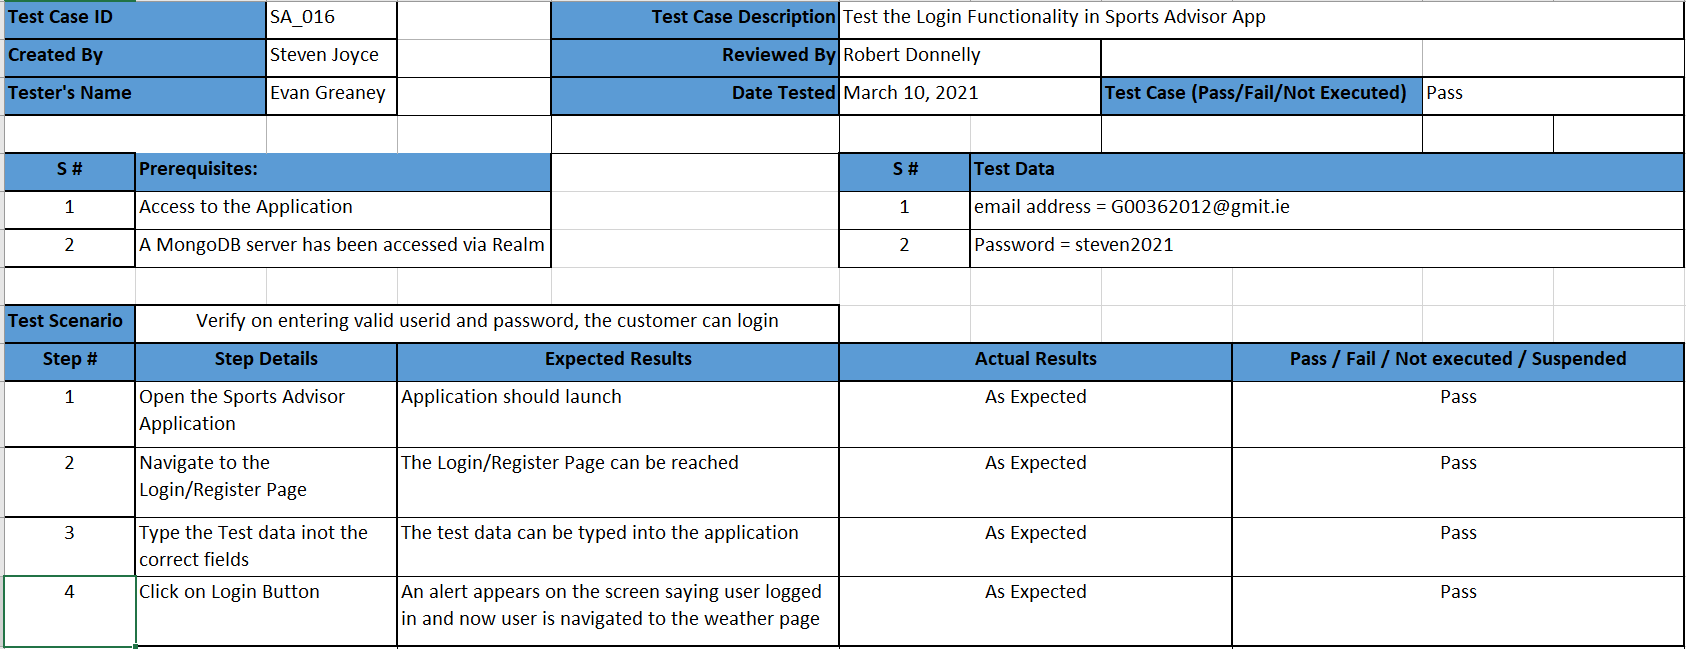
\includegraphics[width=11cm]{img/LoginTestCase.PNG}
    \caption{Test Case for successful Login}
    \label{fig:altas config}
\end{figure}
The image above illustrates the test case we designed and implemented for testing the Login function of our application. The test is designed for a successfully login test. 
\section{Collaborative Platforms}
\subsection{Version Control}
The platform all team members were most familiar with was GitHub, it allows members to access project code versions and commit their contributions to one repository. Every team member has access to view and modify the contents of the repository. All changes are logged and any commit can be accessed at all times , this helps with problem solving as any issues that occur can be called back on to older commits that were functional if issues occur with the latest commit.

\subsection{Communication Tools}
\subsubsection{Microsoft Teams}
Microsoft Teams was used primarily to communicate with our supervisor. We chose this as it is linked to our student accounts and our supervisor requested us to use it as a way to communicate with them. Teams is a good platform for video calls as it can be accessed in multiple platforms such as an Internet browser, Mobile/Desktop Application . It allows users to share files and can sync to your google drive account(file hosting service).and use a calendar feature allowing users to organize meetings.
\newline
However it is not strongly suited for messaging as its forum feature can become cluttered and tedious to navigate,
This is one of the main reasons why we decided to use Discord as our primary form of communication as a team.
\subsubsection{Discord} Discord is a communication Application which has increased in popularity in recent years, especially considering the current pandemic. It runs on Desktop, Mobile and browser platforms. This allowed us to always be in contact with each other if one team members device was running into issues.
\newline
Discord allowed us to set up separate channels to sort our messages to relate to specific aspects of the Project. We could co ordinate and plan different parts of the project in the one place with no clutter, Each aspect of the project had a dedicated channel so that unrelated messages would not be spam our feed. For example we had an "ideas" channel where we would jot down random ideas or inspiration for new features of the application, these messages would be separate from our "session-planning" channel which would strictly contain messages related to our sprint meetings .Due to this feature it became our primary platform to communicate.
\newline
\subsubsection{Whats App}
We used Whats App on our mobile devices to organize our sprint meetings as a team. If for any reason a meeting needed to be held on short notice Whats App was the most efficient way of coordinating a set time.
\subsection{Literature Software}
For the Development of this Dissertation we used Overleaf, we found this Latex text editor the effective way to write up due our previous experience. The Documentation Overleaf provides is well structured which helped us with this aspect of the project. After each person wrote a part of the dissertation it was committed to GitHub, which helped with making sure every member of the team had the appropriate version of the Dissertation.
(GitHub, Discord, Teams)
\section{Technology choices}
When choosing the technology to use in our Application, we decided to use a range of new and innovative technologies ranging from IDEs to server clients that are in different stages of development ranging from Pre-Alpha such as MongoDB Realm Kotlin Integration to Stable development with the Kotlin Language
\subsection{Kotlin}
As a team we wanted to learn a new programming language as a challenge for our project and to increase our skill set as Software Developers. One of our lecturer's during one of our online classes from this module mentioned the Kotlin language. This led us to research this language and understand what it could be used for. We saw that Kotlin was an up and coming language that was primarily used for mobile Applications in Android as of September 2020 with hopes of iOS support being implemented in the near future.
\subsection{Intellij IDEA}
At the start of the college year we were introduced to Intellij in our Distributed Systems module. We soon realised that JetBrains who are the founders of Intellij are also the designers of the Kotlin programming language. With this information we decided to use this as our chosen development environment.
\newline
We soon realised that we had the wrong version of Intellij installed on our devices. We needed to have the Intellij IDEA Ultimate to be able to access a Mongo Database. We got this free with the GitHub Student Developer pack. This was an issue that was unforeseen and time consuming but easily rectified.
\newline
With JetBrains owning both Kotlin and Intellij writing the code was seamless and allowed testing to constantly occur. Intellij allowed the use of an Android mobile phone emulator to run these tests.
\subsection{MongoDB}
MongoDB is a NoSQL database service which allows a user to store data from an application for future use. The data stored can be queried in searches which outputs specific results. These result can be processed by the application and read out to the user. We chose to use MongoDB as our server because of our previous experience of developing applications with it as the back end storage.
\newline
\newline
To use a MongoDB cluster we had to create a Mongo Realm application. This is where the user data can be read into the Kotlin application.
This can also send data to the cluster through this Realm application for storage. Realm reads in a cluster which it has permission to access the stored data through a partition key and clusters data to the Kotlin application.
\subsection{JustInMind}
In order to conceptualize and visualise our applications front end layout we had to begin with prototyping our design. While researching design tools for mobile application development, we came across a prototyping tool called JustInMind.
\newline
\newline
It is a high level prototyping tool used to create high quality wire frames that allow developers to visualise their product in real time before finalizing the design of the mobile application. It assisted us in figuring out how we want the user to navigate the application.
\newline
\newline
The Image as seen in Figure 3.1 shows the designing of the prototype for the login/Sign Up page for the user, it gives a simple understanding of the basic functionality required on this page within the Application.
\newline
\newline
In Figure 3.2 it displays the simplicity of designing features within the page on the App, this image shows how designing a prototype for a drop down menu can be easy to design and how the design feels in correlation to the design of the page.
\newline
\newline
We tried to design the app with different orientations which can be seen in Figure 3.3 which shows the prototype for the recommended days page within the application.

\begin{figure}[H]
    \centering
    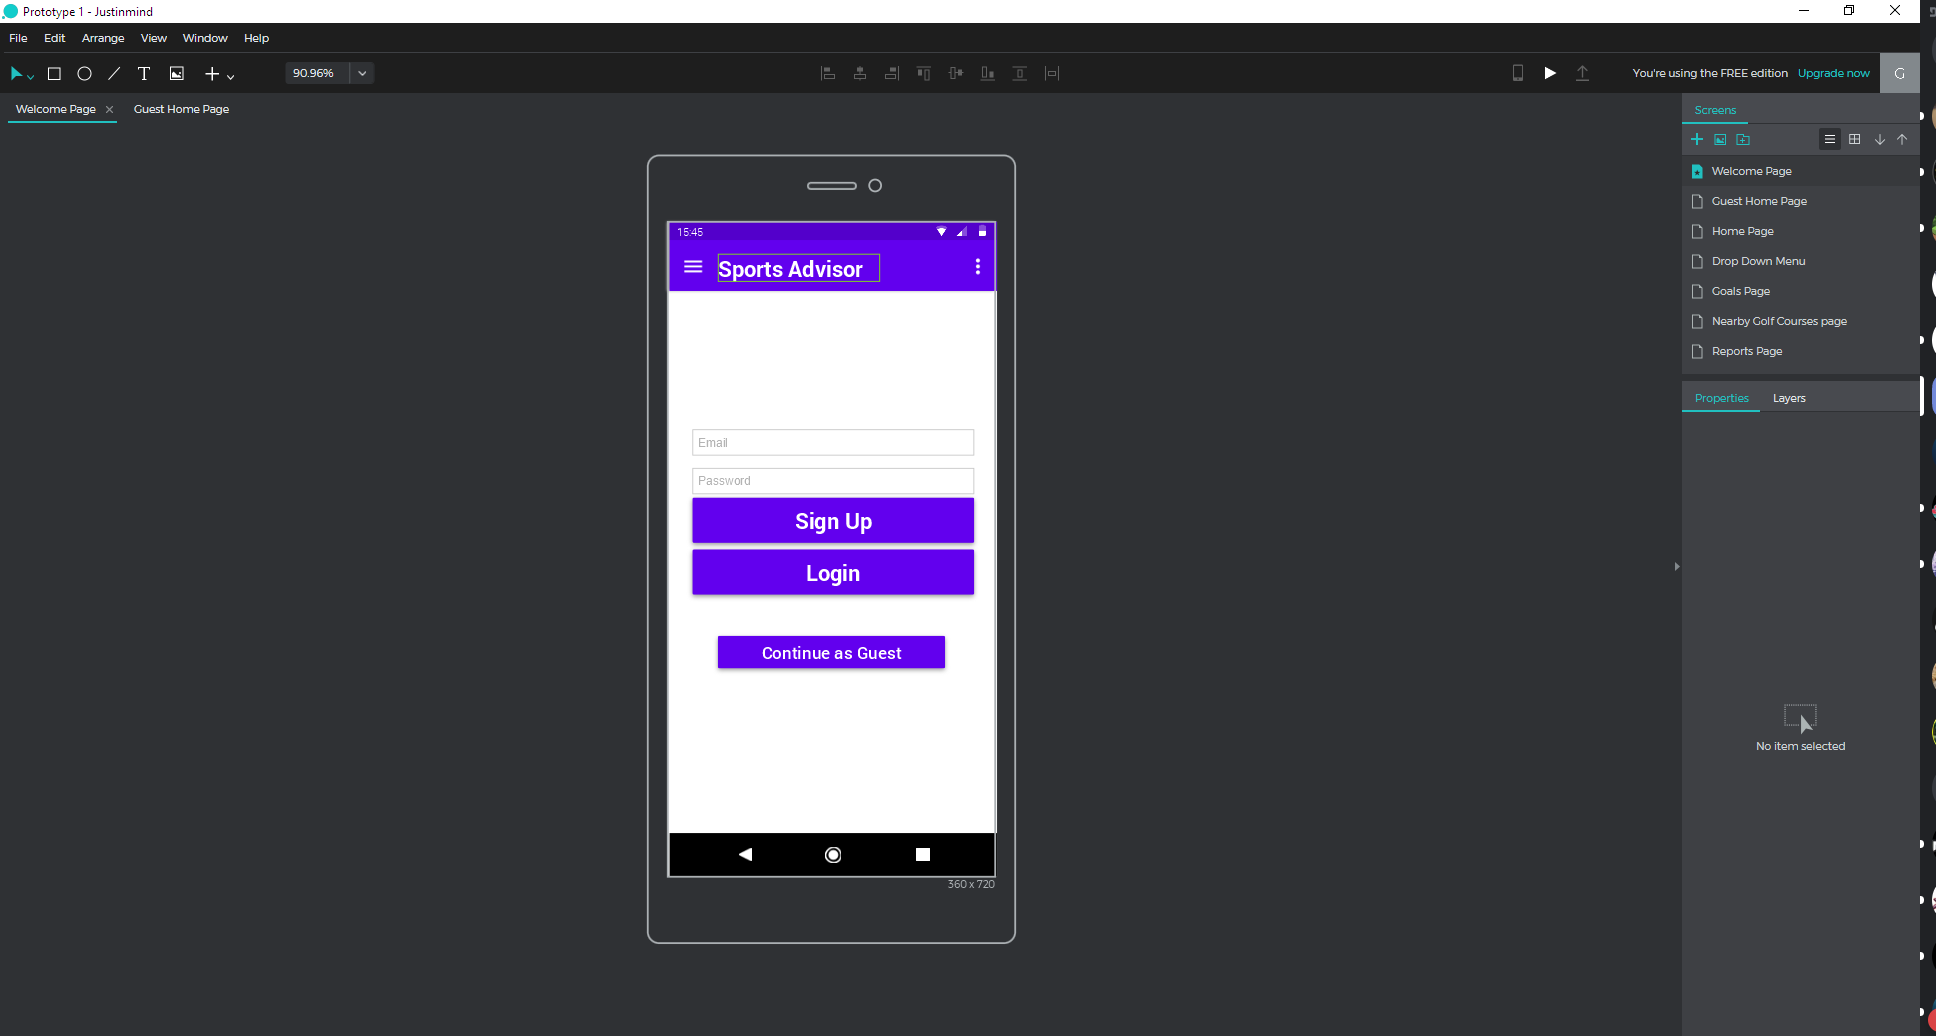
\includegraphics[width=9cm]{img/SignUpImage.PNG}
    \caption{Sign up prototype within JustInMind}
    \label{fig:altas config}
\end{figure}

\begin{figure}[H]
    \centering
    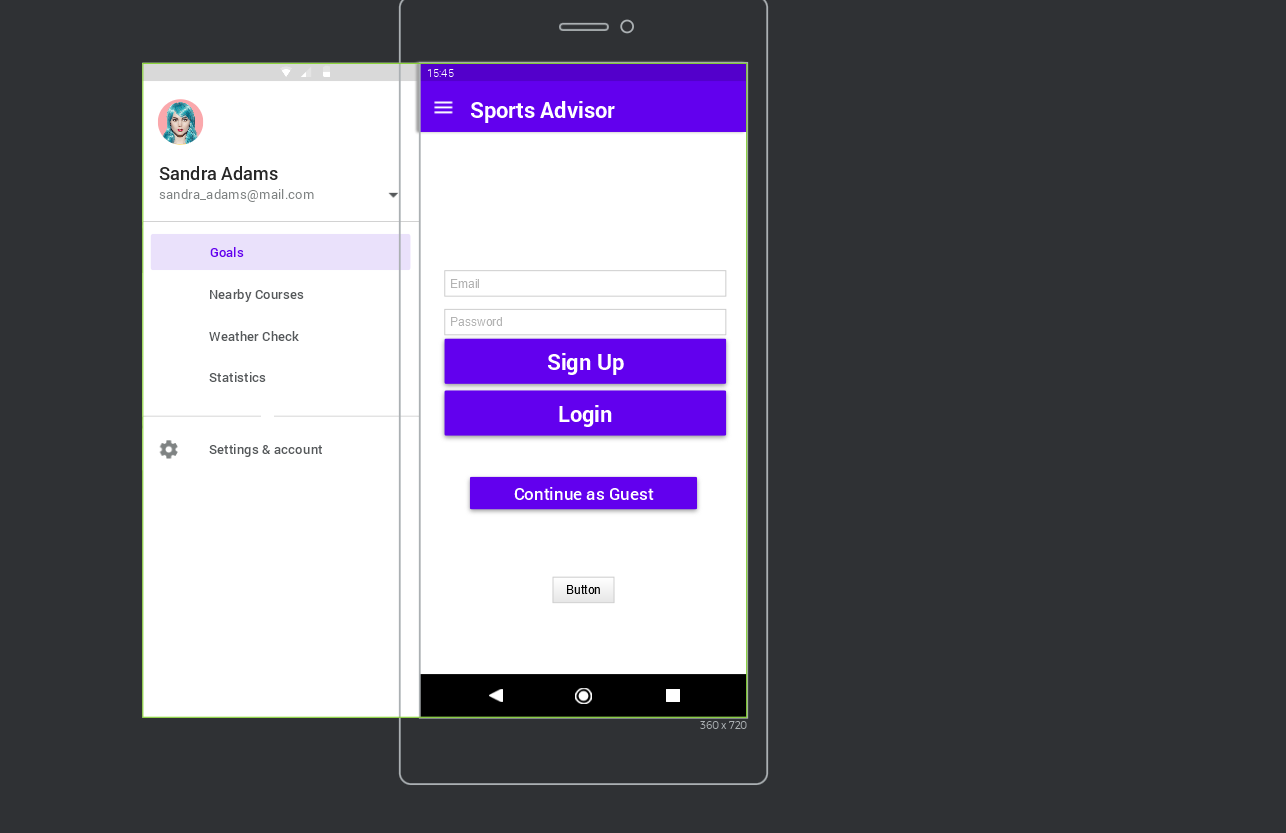
\includegraphics[width=9cm]{img/dropDownMenu.PNG}
    \caption{Drop Down Menu prototype within JustInMind}
    \label{fig:altas config}
\end{figure}

\begin{figure}[H]
    \centering
    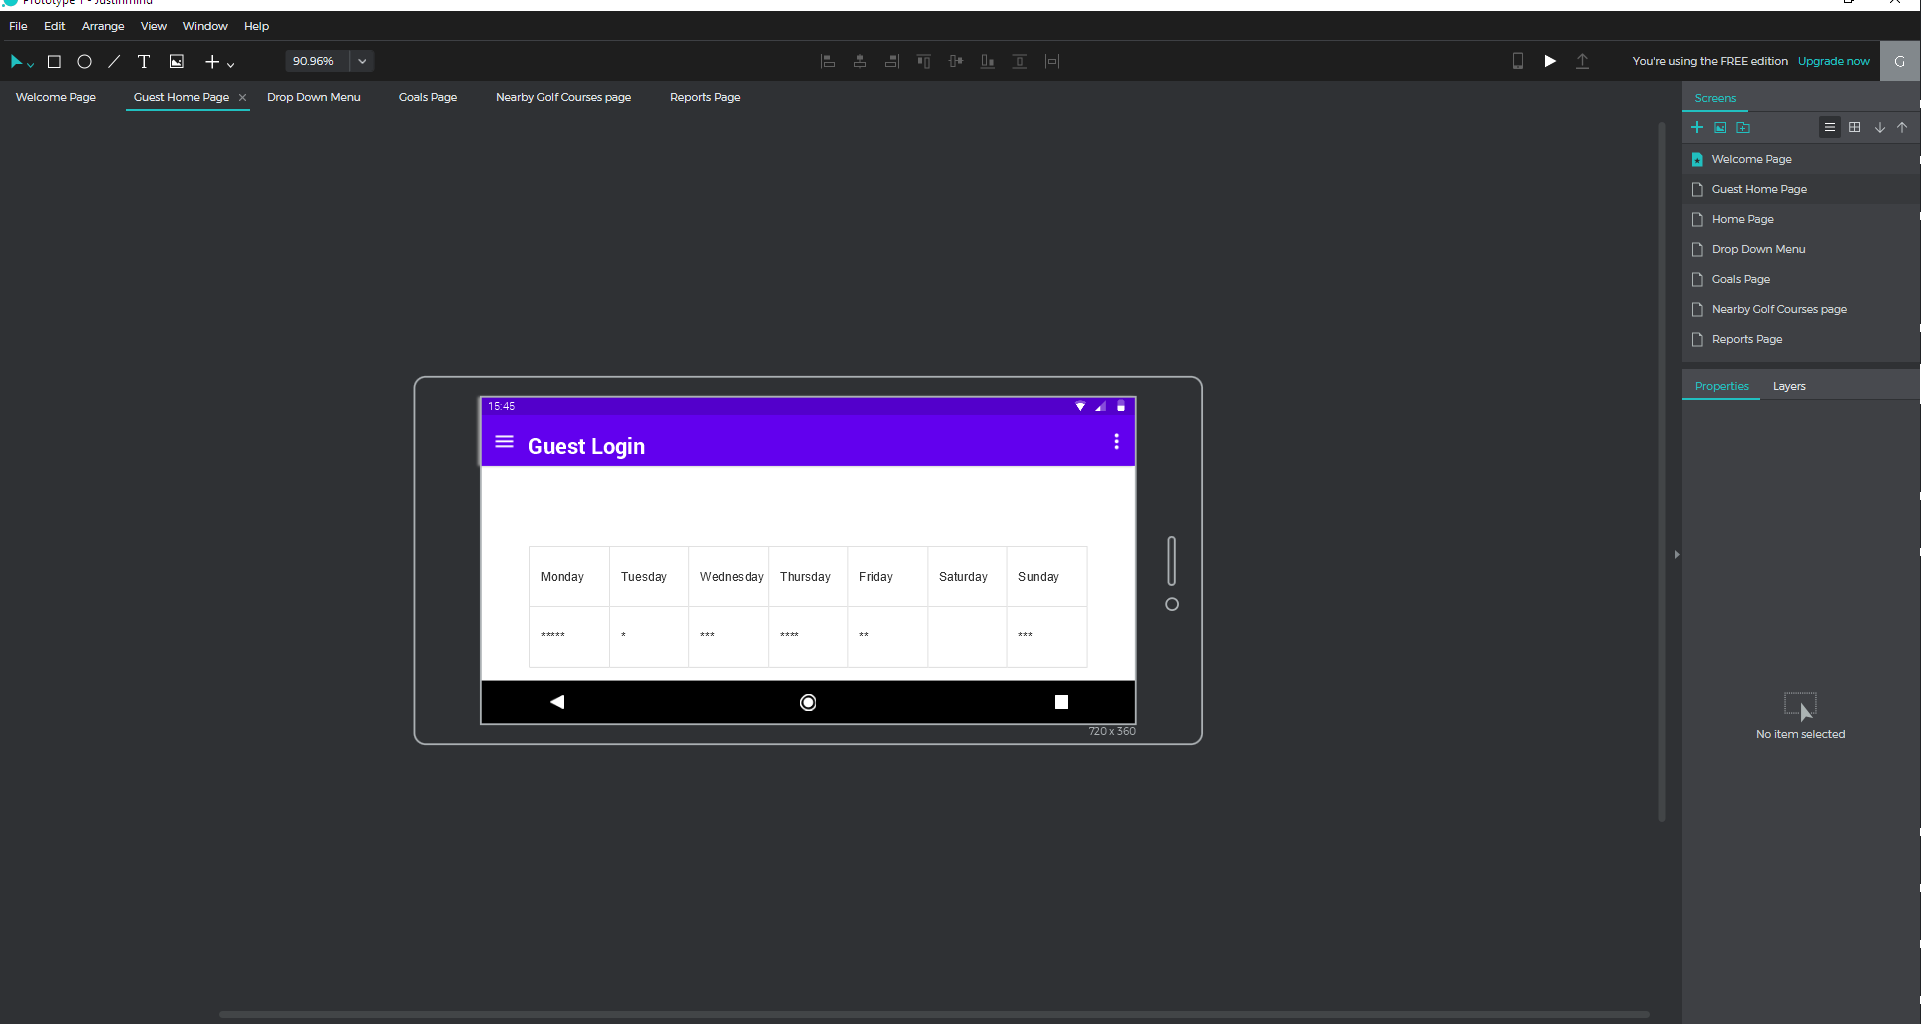
\includegraphics[width=9cm]{img/BestDays.PNG}
    \caption{Best Days to Play prototype within JustInMind}
    \label{fig:altas config}
\end{figure}

\section{Algorithm}
The algorithm we have implemented for the app is used for giving the user feedback on the weather conditions for playing golf during a specific hour on the current date. We generate JSON data from an API call and it contains an abundance of different weather variables which we have saved into variables that can be accessed in the application. We have chosen 8 variables from the list that are key to what hour is best suited to playing a round of golf. They are: sunrise, sunset, hour, amount of rainfall in millimetres, temperature, wind speed and humidity.
\begin{figure}[H]
    \centering
    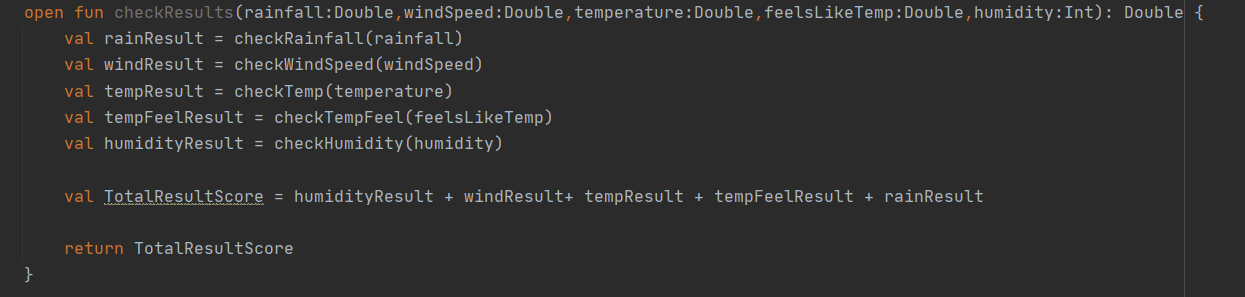
\includegraphics[width=11cm]{img/starRating.PNG}
    \caption{Star rating function}
    \label{fig:altas config}
\end{figure}
All these variables are given back to the user alongside a star rating. The star rating is out of 5, with 0 being the worst and 5 being the best. This is best understood by looking at the above image.


\begin{figure}[H]
    \centering
    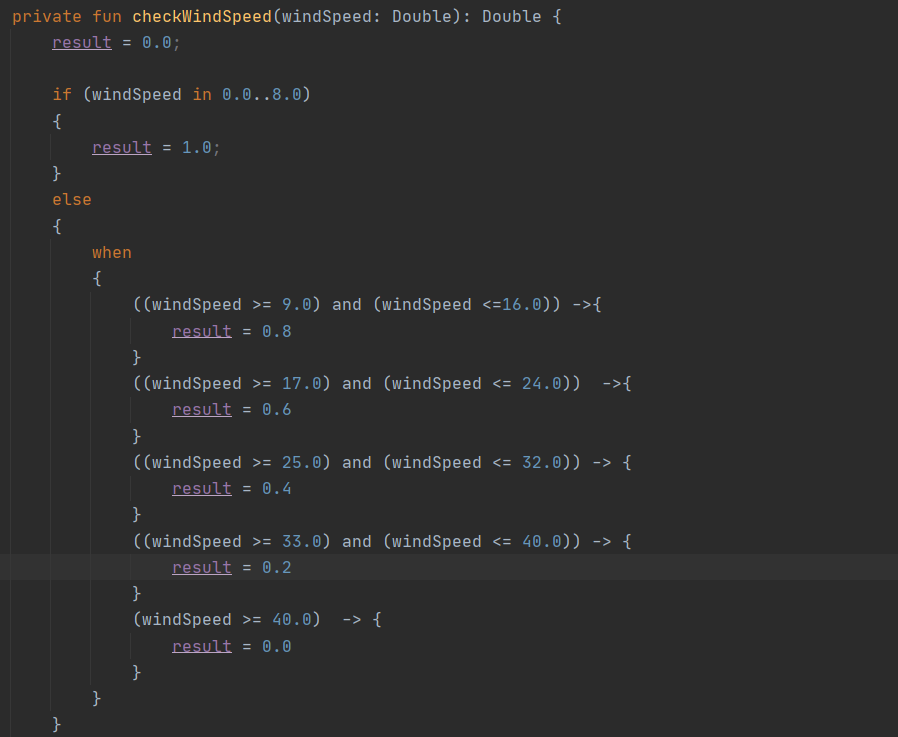
\includegraphics[width=9cm]{img/starEx.PNG}
    \caption{Wind Rating function}
    \label{fig:altas config}
\end{figure}
In the above image we illustrate how we generate a star rating for a variable, every variable is worth 1 star each but that star is broken down into a result between 0 and 1. The result is then used to generate a total score in the check Results function.
\chapter{Technology Review}
\section{Kotlin}
We found Kotlin to be less verbose, easier to read as a programming language compared to such languages as Java, C. It is a high-level language that can be used to produce mobile applications. It's coding style is similar to python but with more features and ways to implement it.  \newline
This is due to Kotlin not needing any end of line syntax to allow the interpreter move on to a new line and code being easier to understand and comprehend what the line of code is doing. - Subject to change
\newline \newline
The Kotlin language is a very good interpreter of other languages which helps when trying to write code without having a great grasp of the language. This is very important when you are beginning to learn the language or when you cannot find a way to write a method in Kotlin that you have done previously in a different language such as Java.
\newline \newline
Despite both Kotlin and Java being a native language for writing Android applications, Kotlin is seen by many as a cleaner and concise way to write code for mobile than Java. It can reduce the amount of lines of code that needs to be written for the application - this comparison can be seen in the code Excerpts below.
\newline
\newline
Below can be seen two examples of code one written in Kotlin and the other in Java, both pieces of code perform the same function but are equally different. As we can see in the Kotlin Code excerpt , the code tends to be more human readable and easier to understand for people less acquainted with either of the languages.
\newline

\subsubsection{Kotlin Code Excerpt}
\begin{verbatim}
    @Throws(IOException::class)
    fun run(url: String?): String? {
        val request: Request = Request.Builder()
            .url(url.toString())
            .build()
        client.newCall(request).execute().use {
        response -> return response.body!!.string()} }
\end{verbatim}
\subsubsection{Java Code Excerpt}
\begin{verbatim}
    OkHttpClient client = new OkHttpClient();
    String run(String url) throws IOException {
        Request request = new Request.Builder()
            .url(url)
            .build();
        try (Response response = client.newCall(request).execute()){
         return response.body().string(); }}
\end{verbatim}

\subsubsection{Limitations of the Kotlin Language}
Kotlin comes with many amazing features that assist the Developer in writing efficient and easy to understand projects and Applications but with all of these innovative and useful tools that come with the Kotlin Language, it is always changing. As the Kotlin programming language is relatively new in comparison to other programming languages such as Java and C++, the language itself and its components vary in stages within a Software release life cycle, an example of which would be the Kotlin/JVM is in stable development since version 1.0 but the component for Multiplatform projects is in Alpha version 1.3 as of the 11th February 2021 which can be seen in Figure 4.1.
\begin{figure}[H]
    \centering
    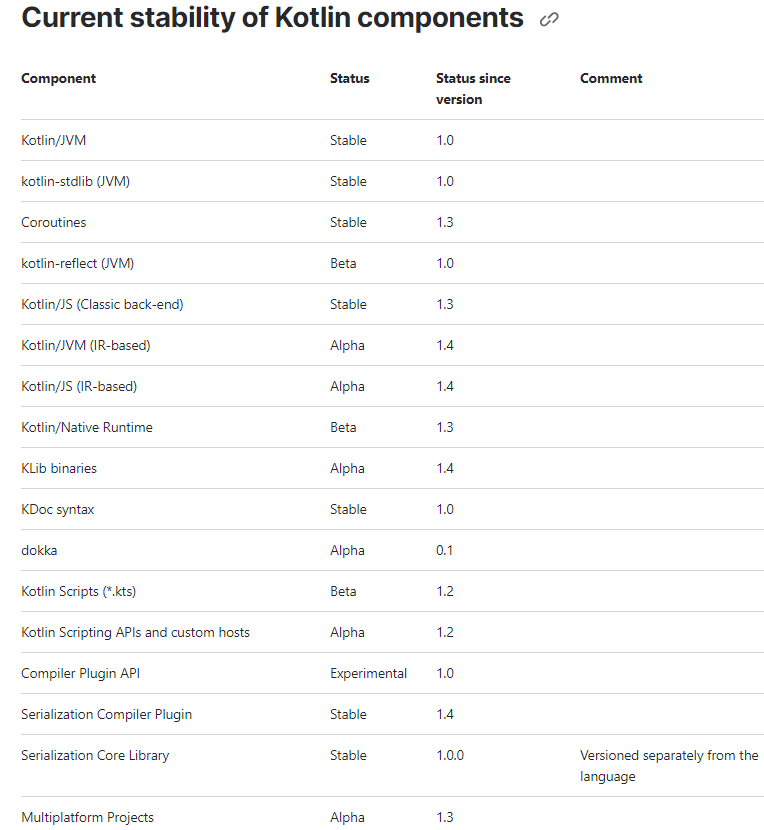
\includegraphics[width=9cm]{img/KotlinStability.PNG}
    \caption{Stability of Kotlin and its components}
    \label{fig:altas config}
\end{figure}
Due to the Multiplatform component not being in a stable release version, we decided to solely focus on development for Android devices as this is included with the stable release of Kotlin/JVM and along with our experience in creating applications for android devices during our time at GMIT.
\newline
\newline
We initially created our base Application with the intention of utilising the multiplatform component for our application. We soon found that it was very difficult to run and in some instances would not compile and would sometimes render the Application completely inoperable. This came as a cause for concern for us in the early stages of development and initially delayed our development by two weeks. It made us reflect on the feasibility of the component and if it would cause major issues later on in the development life cycle of the Application and as a result was ultimately removed from the Application due to being too unstable, with a new project entirely designed for the Android platform being created instead.

\section{Intellij IDEA's}
The development environment provided by Intellij allows for the development of several different types of programs including Mobile Applications. The IDE contains a built in android development environment with Kotlin being the default language. This is due to the development lead designer being Roman Elizarov.
\newline
\begin{figure}[H]
    \centering
    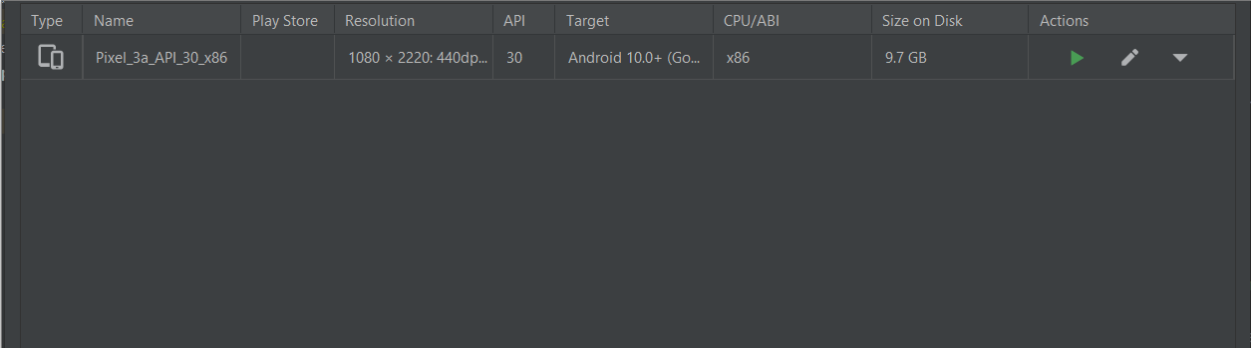
\includegraphics[width=9cm]{img/androidADK.PNG}
    \caption{Android Device Kit}
    \label{fig:adk menu}
\end{figure}
The image above shows the emulated device customisation menu. In here you can add a virtual device to run the android application on. The ability to modify what Android SDK used within the IDE was very important for testing the project. That feature is a great way to debug a mobile application efficiently and in real-time..
\begin{figure}[H]
    \centering
    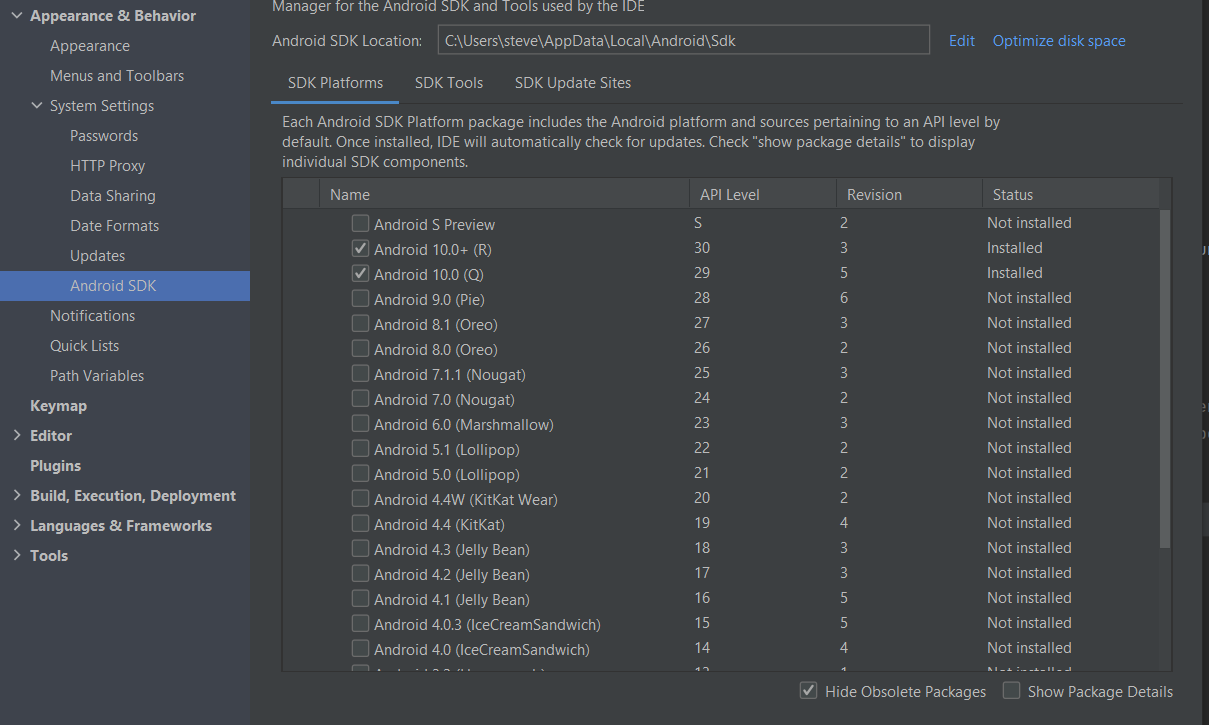
\includegraphics[width=9cm]{img/androidSDK.PNG}
    \caption{Android Software Development Kit}
    \label{fig:sdk menu}
\end{figure}
The SDK manager on Intellij allowed us as developers to run the application on different versions of the Android system. When you choose an SDK, it gives you a percentage of how many people who use Android will be able to use your device. The more up to date version - meant less people could run the app, we when with the Android Oreo version for our virtual phone which is Android 10.0 but we set our minimum SDK version to 28. This allowed the phone to run on Android 9.0(Pie) as well as the version we set up on the virtual device.
\section{API's used}

\subsection{Open Weather API}
Open Weather is an API that allows the user to retrieve weather data from any location using its NWP (Numerical Weather Prediction) Model. This API has been designed to be used universally on any Language to gather data. It gathers this data using a "proprietary convolutional neural network that collects and processes wide range of data sources to cover any location and consider the local nuances of climate." (Quote from "https://openweathermap.org/guide" - Openweather NWP model)

\subsection{Geocoding API}
In order to retrieve data with the Open Weather API, we needed the longitude and latitude of a chosen golf course selected by the user. With the help of the Geocoding API it gives the ability to to convert street name data into longitude and latitude values for the Open Weather API to search weather data based on that location.

\subsection{AccuWeather API}
After a lot of testing and attempting to retrieve data using the Open Weather API and Gecoding API, we found it was very difficult to retrieve,store and convert the data from XML that was provided by the Open Weather API, we then came across the Accuweather API that searches for locations based off of their own location codes which we then use to offer the user a list of golf course locations within Co. Galway that they could choose from instead of having to search for courses themselves.
\newline
\newline
By offering this list we can accurately show the conditions for these particular golf course of choice instead of being able to search for weather conditions for cities and towns instead of the actual golf courses.
\newline
\newline
The data provided from the API is then able to be processed by our Algorithm to provide a rating for the conditions based on two search features, a 12 hour search for that particular day or a search based on next 5 rolling days, the 12 hour search will provide the rating based on the next twelve hours and will provide a rating for those hours, and then the 5 day search will give a general rating for each of the days.  

\section{MongoDB}
To utilise the MongoDB database,we had to use two of its three main core features. The two features we use were Atlas and Realm, Atlas and Realm can be integrated in a way that allows for a seamless connection to and from the Android Application. The MongoDB atlas uses a server that can be either free or paid for use by the a set charge per hour. We choose a free tier server based in N.Virginia (us-east-1) run by Amazon Web Service(AWS). This server was chosen because the Irish server does not work with MongoDB Realm as the server for Ireland is only using MongoDB version is 4.2 but Realm runs on MongoDB version 4.4 and above.
\subsection{Cluster}
It is the word associated with having several MongoDB servers working together.
MongoDB distributes data in 2 ways:replica set and sharded clusters. The main objectives of a MongoDB cluster is to be able to read and write several nodes. The data is separated into the different nodes of the fragment.
\begin{enumerate}
    \item \textbf{Replica Set:}
    \newline This is when the data is sent across several servers without the data changing. This is a layer of protection from a server failure.
    \item \textbf{Sharded Cluster:}
    \newline This is where the data is fragmented into parts of the data to be carried by a different server. This is done to have larger datasets and have better performance.
\end{enumerate}
\subsection{Atlas}
Atlas is the area in which data is stored within the MongoDB system. it allows its users to create a database for a specific user that will only store their data in a collection. \newline This is great for protecting user data. The data can only be accessed by inputting a user id. This user id is unique and is also the user's username that will be always shown in the application. It is the 1st thing a new user will input in the application when creating an account. With the data for a user protected in a cluster, this allows the application to output data to the user that is only relevant to them. That feature was a major reason for using MongoDB in our application.
\newline
The user can store the name of the golf course they played at and the score they got that day. It will also save the par for the course that date and the overall total score for the round of golf. \newline
\begin{figure}[H]
    \centering
    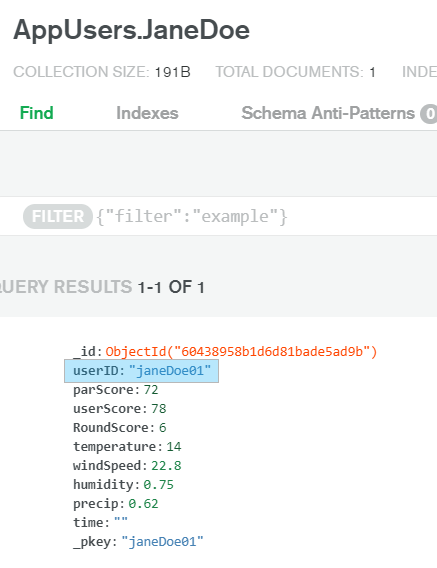
\includegraphics[width=9cm]{img/UserDatabase.png}
    \caption{MongoDB database with a User}
    \label{fig:altas config}
\end{figure}
The highlighted field in the above figure is the authentication key that will need to be inputted by the user to access the database associated with them. Without this key being correctly inputted, the user will not get any data from the MongoDB cluster. This is how MongoDB protects user data.
\subsection{Realm}
The Realm feature of MongoDB is how MongoDB now interprets an Mobile Application. It creates a application that can be used to access a cluster - The cluster is what Atlas creates to store the user data.
\newline
The App will have a unique ID that is called in the Mobile Application back-end to link your application to MongoDB. It creates a user that is linked to a specific database in the cluster.This user can only be authenticated by entering the correct email and password. The app can and does have rules that limit what data a user can access to modify or view.
\newline
\begin{figure}[H]
    \centering
    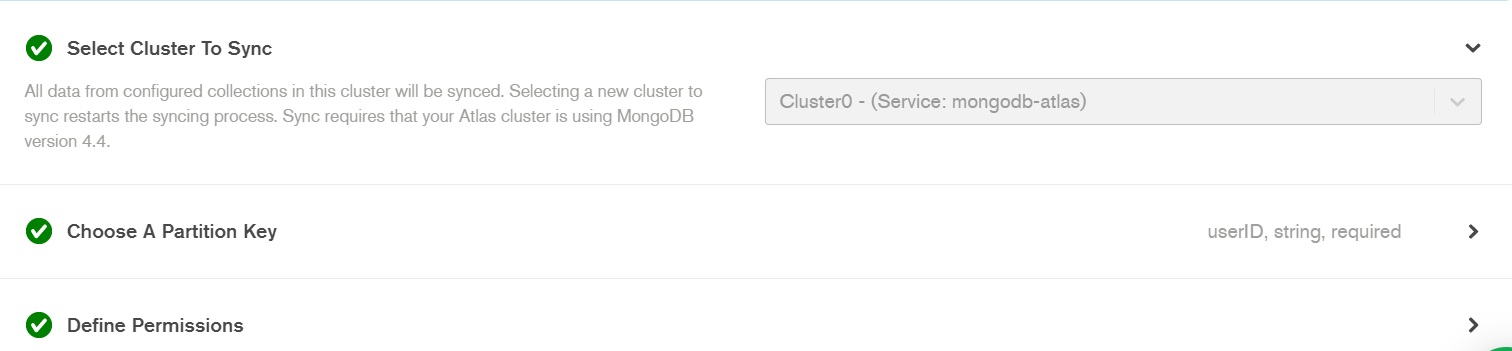
\includegraphics[width=12cm]{img/syncSetup.PNG}
    \caption{MongoDB Sync configuration}
    \label{fig:altas config}
\end{figure}
The above figure is an image of the MongoDB sync configuration. This is where the developer connects to the Atlas cluster by implementing a partition key. This key is how a cluster is made available to the user. The permissions for what a user can do with the database it has connected to is set here as well. We have allowed the user ti both read and write to the collection but the data is protected by the userID key created in the collection itself.

For this project, Realm functioned as the middle man between the application and the MongoDB Server. It allowed the data to be sorted in an manner which is easy to understand and utilize. Despite the Realm Sync still being in a developmental phrase, it is of a high enough standard to work with no issues on their end. We have been contacted by the MongoDB Realm to give feedback to help them see what issues have occurred and if it has worked well for us.

Realm allows the creation of App users. This is the best way we found to make data private and protected. The user will have to login to the server with their username, email and password. These are created in the app and are stored on the Realm App external storage system.
\begin{figure}[H]
    \centering
    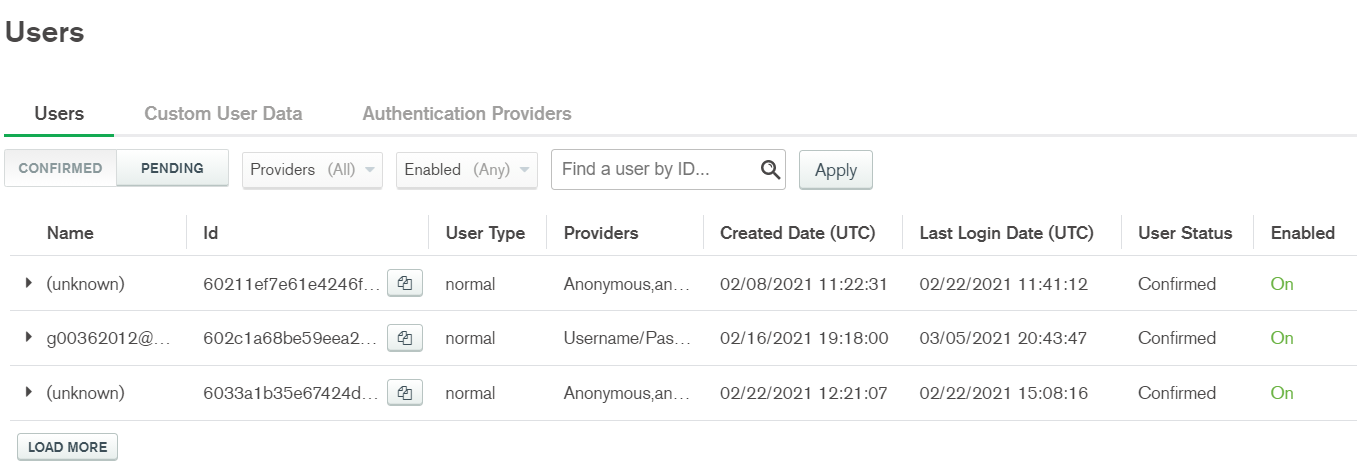
\includegraphics[width=13cm]{img/Users.PNG}
    \caption{MongoDB database with a User}
    \label{fig:altas config}
\end{figure}
The image shown above in figure 4.3 is a snippet of the User database on the Realm App. The realm app will create a temp user for a guest to get a quick api call that shows the weather outlook for next 24 hours. The multi day weather report is only available for users who have logged in.The user needs to login with an email and password.

\section{GitHub}
GitHub is the code hosting platform we used for our project which allows us to track and manage our source code with version control in a collaborative fashion. We used a private repository which allowed us to control who could access our code as well as who could contribute to our code. It allowed us to use branches to merge our code so we can work on separate features and not worry about breaking each others code. Since it is directly connected to git we were able to push and pull code directly from the terminal which we had experience in and as a result was our preference over using Intellij's inbuilt GitHub features. The GitHub website has a solid user interface, the service is stable and reliable so we had no worries about hosting our code on there site. GitHub also offers a student pack which gives students free access to developer tools which we incorporated into our project including Mongo Realm and Intellij Ultimate.
\section{Communication Application's}
\subsection{Discord}
\subsection{Teams}

About seven to ten pages.
\begin{itemize}
\item Describe each of the technologies you used at a conceptual level. Standards, Database Model (e.g. MongoDB, CouchDB), XMl, WSDL, JSON, JAXP.
\item Use references (IEEE format, e.g. [1]), Books, Papers, URLs (timestamp) – sources should be authoritative.
\end{itemize}

\chapter{System Design}
As many pages as needed.
\begin{itemize}
\item Architecture, UML etc. An overview of the different components of the system. Diagrams etc… Screen shots etc.
\end{itemize}
\begin{table}[h]
  \centering
  \begin{tabular}{x{2cm}p{3cm}}
    \toprule \\
    Column 1 & Column 2 \\
    \midrule \\
    Rows 2.1 & Row 2.2 \\
    \bottomrule
  \end{tabular}
  \caption{A table.}
  \label{table:mytable}
\end{table}
\chapter{System Evaluation}
As many pages as needed.
\section{Unit Testing}
\section{Application Deployment}
\section{Application Features}
\section{Objectives Overview}
\section{Issues, limitations}
\section{Future of Application}
\begin{itemize}
\item Prove that your software is robust. How? Testing etc.
\item Use performance benchmarks (space and time) if algorithmic.
\item Measure the outcomes / outputs of your system / software against the objectives from the Introduction.
\item Highlight any limitations or opportunities in your approach or technologies used.
\end{itemize}
\chapter{Conclusion}
About three pages.
\begin{itemize}
\item Briefly summarise your context and objectives (a few lines).
\item Highlight your findings from the evaluation section / chapter and any opportunities identified.
\end{itemize}
\chapter{References}
\chapter{Appendices}
